%\documentclass[10pt,handout]{beamer}
\documentclass[10pt]{beamer}
\usepackage{babel} % Anpassa efter svenska. Ger svensk logga.
\usepackage[utf8]{inputenc} % Anpassa efter linux
\usepackage{graphicx}
\usepackage{../common/beamerthemeUppsala}
%\usetheme{Uppsala}
%\usecolortheme{UU} % Anpassa efter UU:s frger och logga
%\hypersetup{pdfpagemode=FullScreen} % Adobe Reader ska ppna fullskrm
\setbeamertemplate{itemize items}[circle]

% \usepackage{beamerthemesplit}
\usepackage{amsmath}
\usepackage{amssymb}
% \usepackage{graphics}
% \usepackage{graphicx}
% \usepackage{epsfig}
% \usepackage[latin1]{inputenc}
 \usepackage{color}
% \usepackage{fancybox}
% \usepackage{psfrag}
% \usepackage[english]{babel}

\usepackage{array}
%\usepackage{multirow}

 \setbeamertemplate{footline}{\hfill\insertframenumber/\inserttotalframenumber}

% Read in commands
% Course settings
\newcommand{\currentsemester}{Autumn 2024}

% New commands
\newcommand{\bfm}[1]   {\mbox{\boldmath{${#1}$}}}
\newcommand{\Prob}   {\mbox{\textnormal{P}}}
\newcommand{\uured}[1]{\textcolor{uured}{#1}}

% Eqds
\def\eqd{\,{\buildrel d \over =}\,}

% Math operators
\DeclareMathOperator{\E}{\mathbb{E}}
\DeclareMathOperator{\V}{\mathbb{V}}


%%%%%%%%%%%%%%%%%%%%%%%%%%%%%%%%%%%%%%%%%%%%%%%%%%%%%%%%%%%%%%%%%%

\setlength{\parskip}{3mm}
\title[]{{\color{black}Machine learning -- Block 1(b)}}
\author[]{M{\aa}ns Magnusson\\Department of Statistics, Uppsala University}
\date{\currentsemester}


\begin{document}

\frame{\titlepage
% \thispagestyle{empty}
}

%%%%%%%%%%%%%%%%%%%%%%%%%%%%%%%%%%%%%%%%%%%%%%%%%%%%%%%%%%%%%%%%%%


\begin{frame}{This weeks lectures}
\begin{itemize}
\item Regularization
\item Model Selection and Assement
\item Cross-Validation
\item Evaluate classification models
\end{itemize}
\end{frame}


%%%%%%%%%%%%%%%%%%%%%%%%%%%%%%%%%%%%%%%%%%%%%%%%%%%%%%%%%%%%%%%%%%


\section{Predictive Performance}
% What is predictive performance?
\frame{\sectionpage}

\begin{frame}{Previous Model Evaluation}
\begin{itemize}
\item In the past, tools for assessing models, e.g.:
\begin{itemize}
%\item Various plots
\item Residuals
\item Leverage, Cook's distance
\item p-values
\item $R^2$
\item AIC
\item (LOO-CV)
\end{itemize}
\item Model diagnoses and \uured{how well the model fits the data}.
\pause
\item In statistics: focus on \uured{estimation} and \uured{attribution}.
\item In supervised learning: focus on \uured{predictive performance}:
\end{itemize}
\end{frame}


\begin{frame}{Predictive Performance}

% We are looking at predictive performance here


How well our model $\hat{f}_\mathcal{T}$ trained on
\[
\mathcal{T}=\{(y_i, x_i), i = 1, ..., n\}
\]
work when predicting a \uured{new observation} $(y_0,x_0)$ from the data generating process $P_{y,x}$.
\[
\E\left[L(y_0,\hat{f}_\mathcal{T}(x_0))\right] = \int L(y_0, \hat{f}_\mathcal{T}(x_0)) P_{(y,x)} d(y_0,x_0)
\]
where $L(y,x)$ is a \uured{loss function} (e.g. $L(x,y) = (x-y)^2$)

\end{frame}



\begin{frame}{Predictive Performance}
\begin{itemize}
\item ability to perform well on previously unobserved inputs is called \uured{generalization}
\item $\E\left[L(y_0,\hat{f}_\mathcal{T}(x_0))\right]$ is the \uured{generalization error}
\pause
\item Models can be \uured{overfit}%\footnote{See e.g. Picard, R.R., Cook, R.D. (1984). Cross-validation of regression models. \emph{Journal of the American Statistical Association}, \textbf{79(387)}, 575--583.}:
\begin{itemize}
\item explain training data well
\item poor generalizability
\end{itemize}
\pause
\item Models can be \uured{underfit}
\begin{itemize}
\item explain training data poorly
\item poor generalizability
\end{itemize}
\end{itemize}

\end{frame}

\section{Measuring Performance}
\frame{\sectionpage}
% How do we measure predictive performance?

\begin{frame}{Loss Functions}

% We are looking at predictive performance here


\begin{itemize}

\item To assess the performance we use the loss function for a new unseen observation $y_0$ and the prediction of that observation $\hat{f}(x_0)$
\[
L(y_0,\hat{f}(x_0))
\]
\pause
\item This is quite general and we choose based $L$ based on what we want the model performe well on.\pause
\item Examples:
\begin{itemize}
\item Regression problems (squared loss/error):
\[
    L(y_0,\hat{f}(x_0)) = (y_0 - \hat{f}(x_0))^2
\]
\pause
\item Classification (0-1 loss)
\[
    L(y_0,\hat{f}(x_0)) = I(y_0 = \hat{f}(x_0))
\]
\pause
\item In general: The \uured{negative log likelihood} is a good loss function
\end{itemize}


\end{itemize}

\end{frame}


\begin{frame}{Cross-Entropy Loss}

\begin{itemize}
\item When we predict probabilities $\hat{f}(x_0)=\hat{p}$:
\[
L(y_0, \hat{p}) = - (y_0 \log{\hat{p}}) + ((1 - y_0) \log{(1- \hat{p})})
\]
\uured{Question:} Do you recognize the (cross-entropy) loss function?
% Bernoulli negative log-likelihood?
\pause
\item Maximizing the likelihood is the same as minimizing the cross-entropy. \pause
\item Multi class cross-entroy over $M$ classes
\[
L(\mathbf{y}_0, \hat{\mathbf{p}}) = - \sum^M_{j=1} y_{0,j} \log{\hat{p}_j}
\]
\end{itemize}

\end{frame}


\begin{frame}{The Confusion Matrix}

\begin{itemize}
\item A common way to present performance in classification is \uured{the confusion matrix}:
\end{itemize}
\centering
\begin{tabular}{lcc}
  & Prediction &  \\
  Actual & Positive & Negative \\
  Positive & True Positive (TP) & False Negative (FN) \\
  Negative & False Positive (FP) & True Negative ((TN)
\end{tabular}


\end{frame}

\begin{frame}{The Confusion Matrix: Multi-class}

\centering
\begin{tabular}{lccc}
  & Prediction &  \\
  Actual & a & b & c \\
  a & $T_a$ & $F_{ab}$ & $F_{ac}$ \\
  b & $F_{ba}$ & $T_b$ & $F_{bc}$ \\
  c & $F_{ca}$ & $F_{cb}$ & $T_c$ \\
\end{tabular}
and
\centering
\begin{tabular}{lccc}
  & Prediction &  \\
  Actual & TP & FP & FN \\
  a & $T_a$ & $F_{ba} + F_{ca}$ & $F_{ab} + F_{ac}$ \\
  ... & ... & ... & ...
\end{tabular}
and $N$ is the sum over all cells.



\end{frame}


\begin{frame}{Accuracy}

% We are looking at predictive performance here

\[
\text{Accuracy} = \frac{(\text{TP+TN})}{\text{(TP+FP+FN+TN)}}
\]

or

\[
\text{Accuracy} = \frac{T_a + T_b + T_c}{N}
\]

\pause


\uured{Question}: Can you see a problem with Accuracy?
% Unbalanced samples

\end{frame}

\begin{frame}{Precision}

Of all the predicted positives, how many are \uured{actually positive}?

% Want to use when want to be sure about a prediction
\[
\text{Precision} = \frac{(\text{TP})}{\text{(TP+FP)}}
\]
or
\[
\text{Precision}_a = \frac{(T_a)}{T_a + F_{ba} + F_{ca})}
\]

All \uured{predicted} $a$: $T_a + F_{ba} + F_{ca}$

If we want one precision estimate for all classes:
\begin{enumerate}
\item Macro-average ($\text{Precision}_a, ..., \text{Precision}_c$)
\item Micro-average (use Table 2)
\end{enumerate}

\end{frame}



\begin{frame}{Recall}

% Want to use when want to be sure about a prediction
Of all \uured{positives}, how many are predicted correctly (recalled)?\pause

\[
\text{Recall} = \frac{(\text{TP})}{\text{(TP+FN)}}
\]
and
\[
\text{Recall}_a =  \frac{(T_a)}{T_a + F_{ab} + F_{ac})}
\]

All \uured{true/actual} $a$: $T_a + F_{ab} + F_{ac}$

If we want one precision estimate for all classes:
\begin{enumerate}
\item Macro-average ($\text{Recall}_a, ..., \text{Recall}_c$)
\item Micro-average (use Table 2)
\end{enumerate}



\end{frame}

\begin{frame}{Sensitivity and specificity}

\[
\text{Sensitivity} = \text{Recall of \uured{positive} class} =  \frac{\text{TP}}{\text{TP+FN}}
\]
and
\[
\text{Specificity} = \text{Recall of \uured{negative} class} =\frac{\text{TN}}{\text{TN+FP}}
\]

\end{frame}


\begin{frame}{F1-score}

% Want to use when want to be sure about a prediction
Harmonic mean of Precision and Recall.

% F1: Both good precision and recall
\[
\text{F}_1 = \frac{2}{\text{Precision}^{-1} + \text{Recall}^{-1}} = 2 \cdot \frac{\text{Precision} \cdot \text{Recall}}{\text{\text{Precision} + \text{Recall}}}
\]
\uured{Question}: What happens if Precision or Recalls goes toward zero/one?
\pause
Very common performance measurement in practice.

If we want one precision estimate for all classes:
\begin{enumerate}
\item Macro-average ($\text{F}_{1a}, ..., \text{F}_{1c}$)
\item Micro-average (use Table 2)
\end{enumerate}

\end{frame}



\begin{frame}{Example}

Say that we want to classify spam vs. ham. \\[3mm]\pause
%TODO: Images here

\begin{center}
\begin{tabular}{ l | c | c }
  & $\hat{f}(x)=1$ & $\hat{f}(x)=0$\\
  \hline
  $y=1$ & 515 & 91 \\
  $y=0$ & 85 & 569 \\
  \hline
\end{tabular}
\end{center}
The cell counts yield us estimates of
\begin{enumerate}
\item Accuracy: $\frac{515+569}{515+91+85+569}\approx 0.86$
\item Precision: $\frac{515}{515+85}\approx 0.86$
\item Recall: $\frac{515}{515+91}\approx 0.85$
\item $F_1$: $\frac{2 \cdot 0.85 \cdot 0.86}{0.85 + 0.86}\approx 0.855$
\end{enumerate}

\pause

In this example, we let $\hat{y}_i=1$ whenever $\hat{\pi}_i>0.5$.

What if we choose another cut-off level $\hat{\pi}_i>\alpha$ instead?

\end{frame}


\begin{frame}{Classification tables}

\begin{center}
\begin{tabular}{ l | c | c }
 {\color{uured}$\alpha=0.5$} & $\hat{f}(x)=1$ & $\hat{f}(x)=0$\\
  \hline
  $y=0$ & 515 & 91 \\
  $y=1$ & 85 & 569 \\
  \hline
\end{tabular}
\end{center}
\pause
Now let $\alpha=0.3$ instead, so that we are more prone to say that $\hat{y}=1$:
\begin{center}
\begin{tabular}{ l | c | c }
  {\color{uured}$\alpha=0.3$} & $\hat{f}(x)=1$ & $\hat{f}(x)=0$\\
  \hline
  $y=1$ & 462 & 144 \\
  $y=0$ & 38 & 616 \\
  \hline
\end{tabular}
\end{center}
The cell counts yield us estimates of
\begin{enumerate}
\item Accuracy: $\frac{462+616}{462+38+144+616}\approx 0.86$
\item Precision: $\frac{462}{462+38}\approx 0.92$
\item Recall: $\frac{462}{462+144}\approx 0.76$
\item $F_1$: $\frac{2 \cdot 0.92 \cdot 0.76}{0.92 + 0.76}\approx 0.83$
\end{enumerate}

The Precision has increased, but the Recall has decreased...

\end{frame}



\begin{frame}{A more problematic example}
A highly unbalanced example. 1001 ham and 17 spam.

Our new classifier: Everything is ham!\pause

\begin{center}
\begin{tabular}{ l | c | c }
  & $\hat{f}(x)=1$ & $\hat{f}(x)=0$\\
  \hline
  $y=1$ & 1001 & 0 \\
  $y=0$ & 17 & 0 \\
  \hline
\end{tabular}
\end{center}
\pause
The cell counts yield us estimates of
\begin{enumerate}
\item Accuracy: $\frac{1001}{1001+17}\approx 0.99$
\item Precision: $\frac{1001}{1001+0}\approx 1.0$
\item Recall: $\frac{1001}{1001+17}\approx 0.99$
\item $F_1$: $\frac{2 \cdot 1 \cdot 0.99}{0.99 + 1}\approx 0.99$
\pause
\item $F_1$ for negative class: $\frac{2 \cdot 0 \cdot 0}{0 + 0}$ Not defined, but 0 in the limit as Precision and Recall goes to 0.
\item And Specificity is 0!
\end{enumerate}

\end{frame}




\begin{frame}<handout:0>{Questions?}
Questions?
\end{frame}

%%%%%%%%%%%%%%%%%%%%%%%%%%%%%%%%%%%%%%%%%%%%%%%%%%%%%%%%%%%%%%%%%%

% Im here

\section{Test and training error}
\frame{\sectionpage}

\begin{frame}{Test Error}

\begin{itemize}
\item The main error of interest - \emph{generalization error}
\item Conditional Test Error \\(Performance for the model trained on \uured{actual} training data):
\[
\text{Err}_\mathcal{T} = \E_{p(X_0,Y_0)}(L(Y_0,\hat{f}(X_0) | \mathcal{T})
\]
\item Expected Test Error \\(Model performance over \uured{different} training datasets):
\[
\text{Err} = \E_{p(X,Y)}(L(Y_0,\hat{f}(X_0)))
\]
\item Sometimes refered to as \uured{generalization} error.
\item Conditional Test Error is more difficult to estimate than the Expected Test Error (Bates, Hastie, and Tibshiriani, 2021)
\end{itemize}

\end{frame}


\begin{frame}{Training Error}

\begin{itemize}
\item Training error: The loss the algorithm try to \uured{minimize}
\item The Error in the training data:
\[
\overline{\text{err}} = \frac{1}{N} \sum_{i=1}^N L(y_i,\hat{f}(x_i))
\]
where $L(y,x)$ is the loss function.

\end{itemize}

\end{frame}


\begin{frame}{Model complexity/capacity}

\begin{itemize}
\item Model complexity/capacity: \uured{The flexibility of the model.}
\item \uured{Underfitting}: Too \uured{low} capacity of model
\item \uured{Overfitting}: Too \uured{high} capacity of model
\item Example: Polynomial regression with higher order terms
\end{itemize}

\begin{figure}[h]
\caption{Model complexity (Goodfellow et al, 2017, Figure 5.2)}
\centering
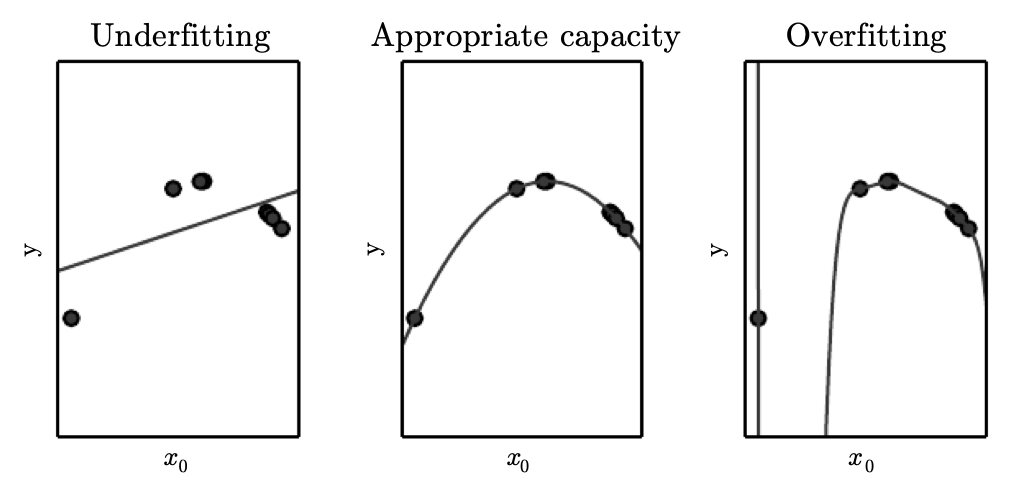
\includegraphics[width=0.9\textwidth]{figs/Dl_5_2}
\end{figure}

\end{frame}


\begin{frame}{Training, test, and complexity}


\begin{figure}[h]
\caption{Test, training, and model complexity (Goodfellow et al, 2017, Figure 5.3)}
\centering
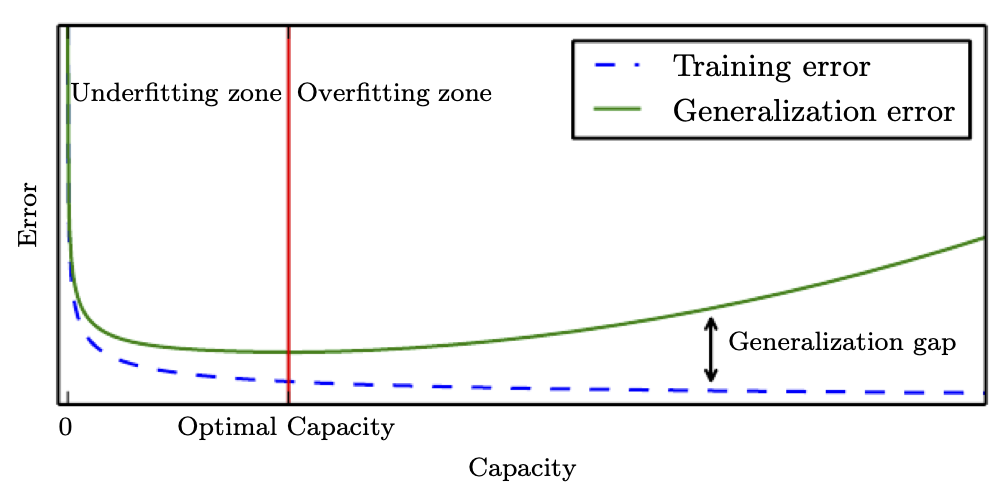
\includegraphics[width=0.8\textwidth]{figs/Dl_5_3.png}
\end{figure}

\end{frame}


\section{Estimating the test error}

\begin{frame}{How to estimate the Test Error (Model Assesment)}

\begin{itemize}
\item We set aside a \uured{test set} from the data
\item Use as the last step to \uured{estimate} the \uured{generalization error}
\item Should only be used \uured{ONCE} (or a few times)\pause
\item Size of testset:
\begin{itemize}
\item Common suggestion is 10\%, but
\item It is a statistical estimation problem (choice of sampling size)
\end{itemize}
\end{itemize}

\end{frame}


\begin{frame}{Multiple Use of Test Set for Model Assesment}

\begin{itemize}
%\item Say that we have $\hat{L}(\mathcal{T})$ an estimate of the loss on the test set given a training set
%\item Lets say that we have $i \in \{1,...,M\}$ be models trained on $M$ independent training sets $\mathcal{T}_i$ but they all have the same underlying error $L^*$
%\item Then we can assume that
%\[
%\hat{L}_i(\mathcal{T}_i) \sim N(L^*, \sigma)
%\]
\item What happens if we use the test set to pick the model?

\end{itemize}

\end{frame}

\begin{frame}<handout:0>{Questions?}
Questions?
\end{frame}

%%%%%%%%%%%%%%%%%%%%%%%%%%%%%%%%%%%%%%%%%%%%%%%%%%%%%%%%%%%%%%%%%%


%\section{Model Selection}
%\frame{\sectionpage}


%\begin{frame}{Model Selection}
%\begin{itemize}
%\item We want to select a model based on performance.
%\item Important when using hyperparameters (as in regularization)
%\end{itemize}

%\end{frame}


\section{Bias and Variance}
\frame{\sectionpage}

\begin{frame}{Bias and Variance}

Assume we have the following data generating process:
\[
Y = f(X) + \epsilon\,,
\]
where $\E(\epsilon)=0$ and $V(\epsilon)=\sigma_\epsilon$.

We have an estimated model $\hat{f}$ and want to predict a new, unseen, observation $x_0$. The error can then be decomposed into:

\begin{align*}
\text{Err}(x_0) &= \E\{(Y-\hat{f}(x_0))^2 | X = x_0\} \\
  &= \sigma^2_\epsilon + \{\E(\hat{f}(x_0)) - f(x_0)\}^2 + \E\{\hat{f}(x_0) - \E(\hat{f}(x_0))\}^2 \\
  &= \sigma^2_\epsilon + \text{Bias}^2(\hat{f}(x_0)) + V(\hat{f}(x_0))
\end{align*}
\pause
\begin{itemize}
\item \emph{Bias}: How close can $\hat{f}$ get to the true model $f$
\item \emph{Variance}: The variability of the predictions from $\hat{f}$
\item \emph{Irreducible/Bayes error}: The minimum possible error
\end{itemize}

\end{frame}


\begin{frame}{Bias and Variance: Linear regression}

In linear regression we have:
\[
\hat{f}(x_i) = \hat{\beta} x_i
\]

This give us the following error decomposition:

\begin{align*}
\frac{1}{N}\sum^N_i \text{Err}(x_i) &= \sigma^2_\epsilon + \frac{1}{N}\sum^N_i (f(x_i) - E(\hat{f}(x_i))^2 + \frac{p}{N} \sigma^2_\epsilon
\end{align*}

\end{frame}


\begin{frame}{Bias and Variance}

\begin{figure}[h]
\caption{Test, training, and model complexity (Hastie et al, 2009, Figure 7)}
\centering
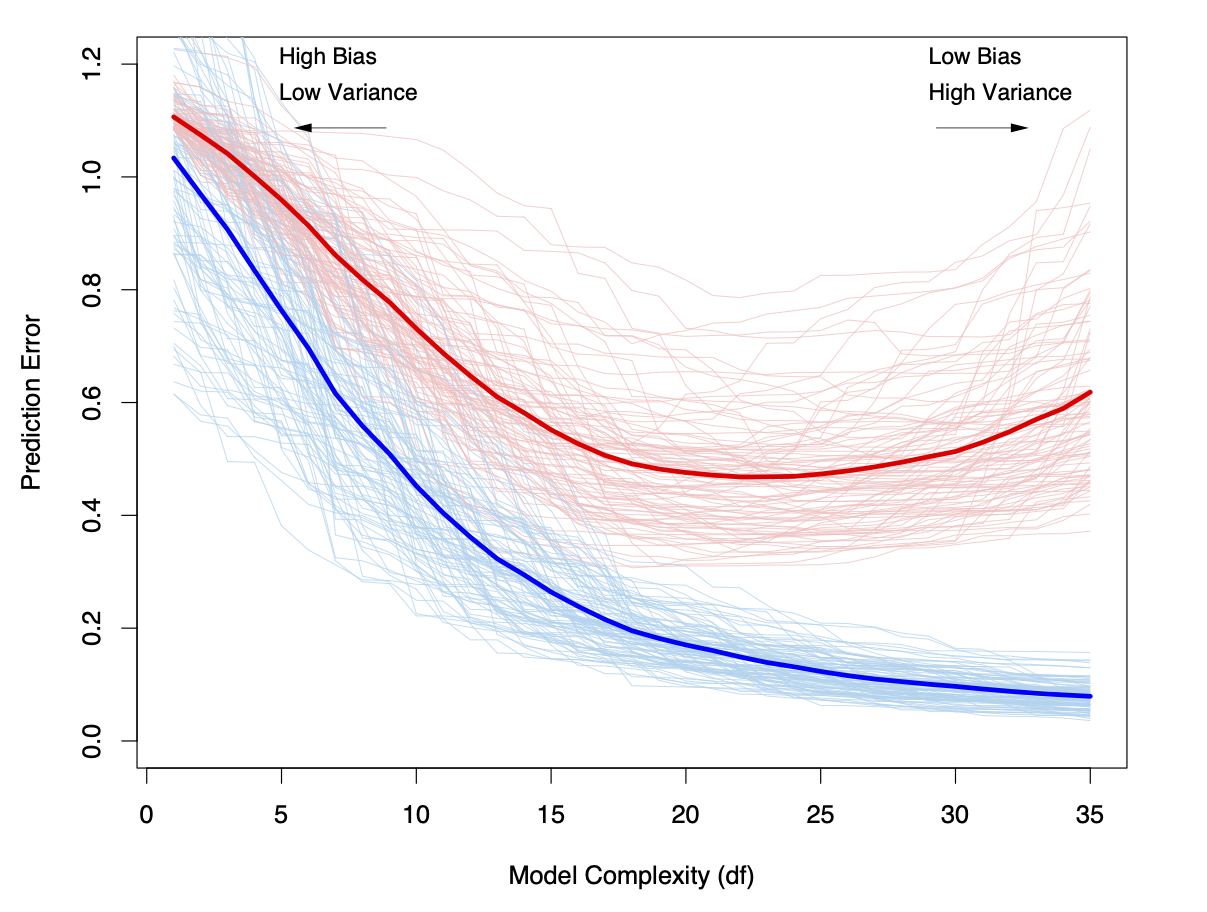
\includegraphics[width=0.65\textwidth]{figs/ESL_7_1.png}
\end{figure}

\begin{itemize}
\item High Bias: \uured{Underfit}
\item High Variance: \uured{Overfit}
\item High Irreducible error: No model is good
\end{itemize}

\end{frame}


\begin{frame}{Bias and Variance}

\begin{figure}[h]
\caption{Bias and variance (Goodfellow et al., 2017, Figure 5.6)}
\centering
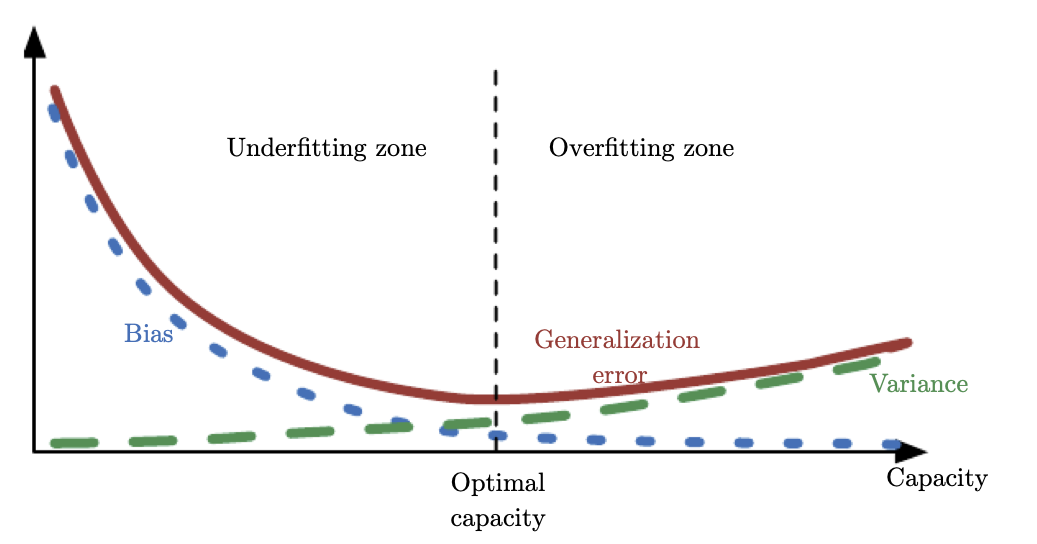
\includegraphics[width=0.9\textwidth]{figs/Dl_5_6.png}
\end{figure}

\end{frame}

%\subsection{Optimism of Training Error}

\begin{frame}{Optimism and training error}

The in-sample \uured{test} error:
\[
\text{Err}_\text{in} = \frac{1}{N}\sum^N_{i=1} \E_{Y^0}\{L(Y^0_i,\hat{f}(x_i))|\mathcal{T}\}\,,
\]
where $Y^0_i$ is a \uured{new variable conditioned on $x_i$}.\\[3mm]
\pause
We have that for many loss functions
\[
\E_\mathbf{y} (\text{Err}_\text{in}) = \E_\mathbf{y}(\overline{\text{err}}) + \underbrace{\frac{2}{N}\sum^N_{i=1} \text{Cov}(\hat{f}(x_i),y_i)}_{\text{optimism}}\,,
\]
or
\[
\text{op} = \E_\mathbf{y} (\text{Err}_\text{in}) - \E_\mathbf{y}(\overline{\text{err}})
\]
where $\overline{\text{err}}$ is the training error.

As $\hat{f}(x_i) \rightarrow y_i$, optimism will increase.

\uured{Question}: Why?


\end{frame}

\begin{frame}{Estimating Optimism}

\begin{itemize}
\item Under certain conditions we can estimate this optimism.
\item AIC is an example of this -- asymptotic predictive performance.
\pause
\item \uured{Question}: What is the optimism in the Figure below?
\end{itemize}


\begin{figure}[h]
\caption{Test, training, and model complexity (Hastie et al, 2009, Figure 7)}
\centering
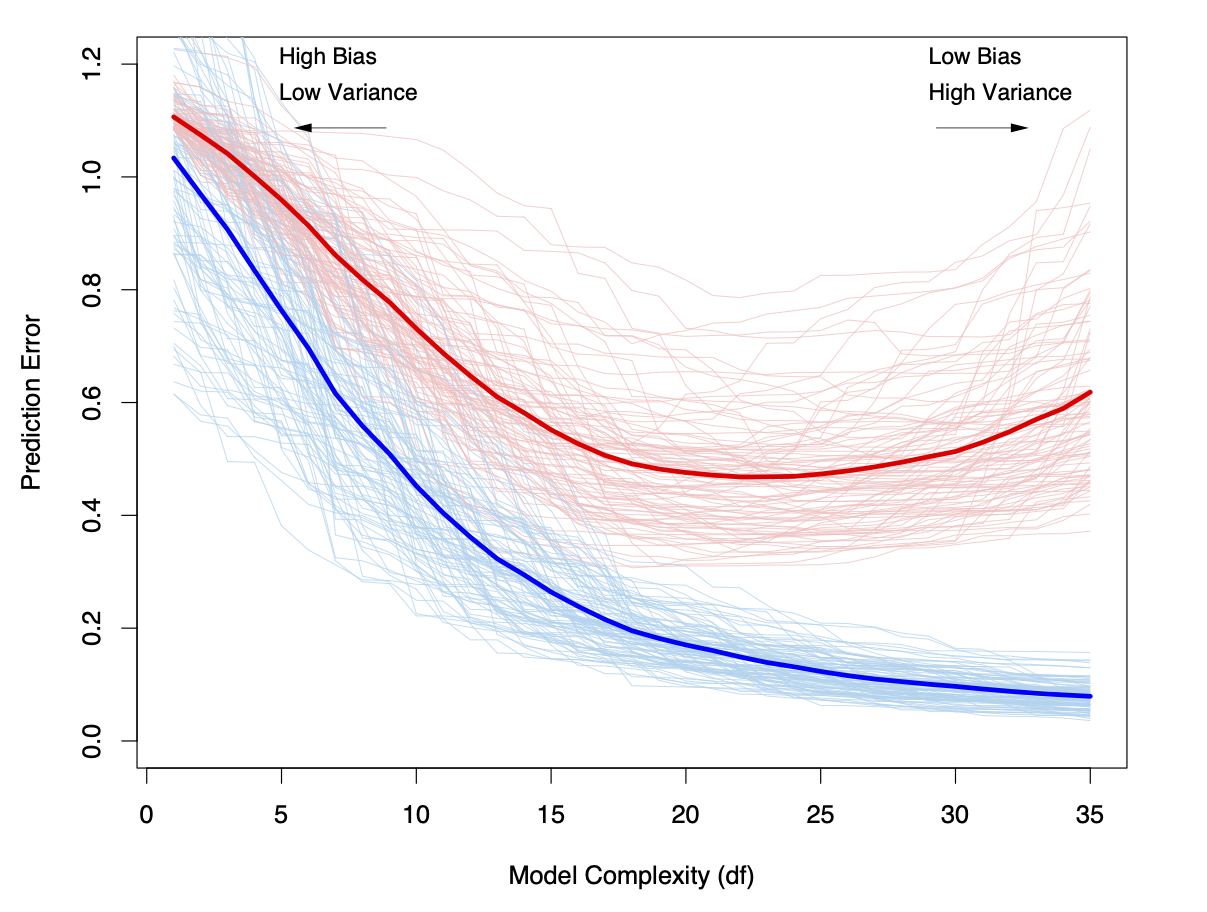
\includegraphics[width=0.65\textwidth]{figs/ESL_7_1.png}
\end{figure}

% Answer the diff between the red and blue line

\end{frame}



\begin{frame}{The double descent of large models}

\begin{figure}[h]
\caption{The double descent of large models (Nakkiran et al., 2019)}
\centering
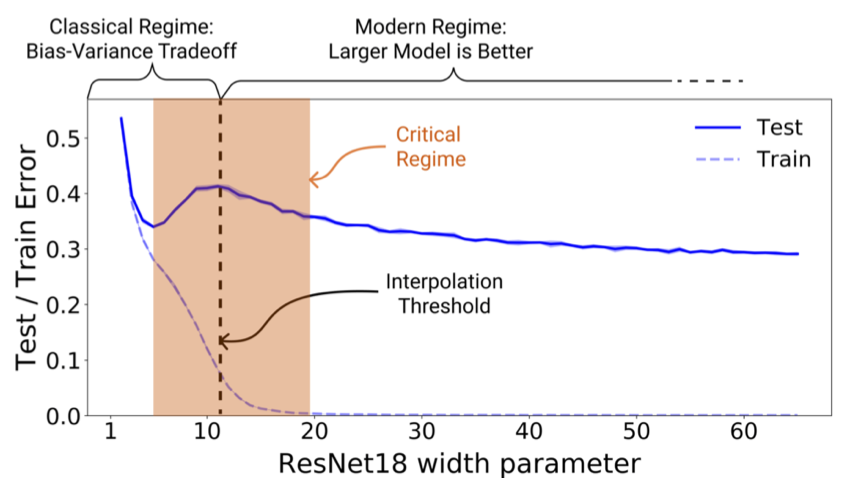
\includegraphics[width=0.9\textwidth]{figs/Nakkiran_et_al_2019.png}
\end{figure}



\end{frame}


\begin{frame}<handout:0>{Questions?}
Questions?
\end{frame}

%%%%%%%%%%%%%%%%%%%%%%%%%%%%%%%%%%%%%%%%%%%%%%%%%%%%%%%%%%%%%%%%%%

\section{Cross-validation}
\frame{\sectionpage}


\begin{frame}{Cross-Valdidation}






\begin{itemize}
\item We want to estimate \uured{$\text{Err}$} for different models and to \uured{choose the best model} where
\begin{align*}
\text{Err} & = \E_{p(X,Y)} (\text{Err}_\mathcal{T}) \\
 & = \E_{p(X,Y)} (\E_{p(X_0,Y_0)}(L(Y_0,X_0)|\mathcal{T})) %\\
% & = \int (\int L(Y_0, \hat{f}(X_0)) p(X_0,Y_0) d(Y_0,X_0) | \mathcal{T}) p(X,Y) d(X,Y)
\end{align*}
\item Cross-Validation is probably the most popular approach to estimate \uured{$\text{Err}$} and choose between models because it is:
\begin{enumerate}
\item Conceptually easy to understand
\item Easy to implement
\item No need for rules-of-thumbs to verify that it is applicable
\item Equally useful for many different type of models
\item Flexible for the use case at hand
\end{enumerate}
\pause
\item Common approach to \uured{learn hyper parameters}\\(that is a model choice)
\end{itemize}

\end{frame}


\begin{frame}{The Cross-Valdidation Algorithm}

\begin{figure}[h]
\caption{Cross-Validation (Hastie et al, 2009, p. 222, 242)}
\centering

\includegraphics[width=0.6\textwidth]{figs/ESL_test_train_val.png}
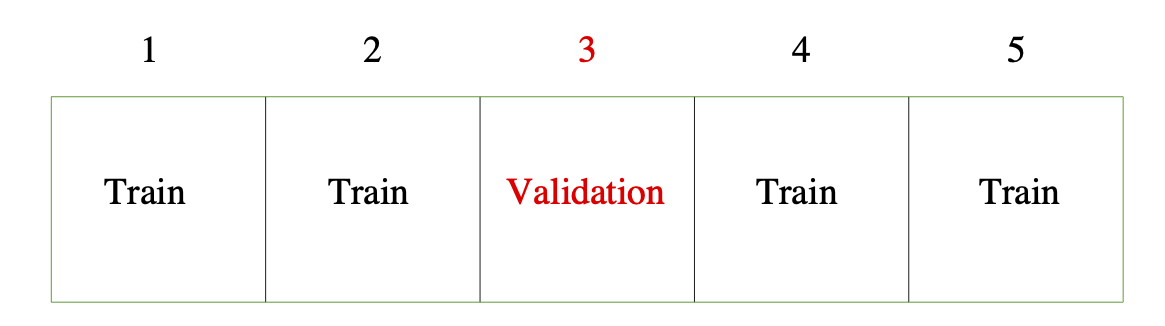
\includegraphics[width=0.6\textwidth]{figs/ESL_cross_val.png}
\end{figure}

\begin{enumerate}
\item Split data in $K$ folds
\item For each fold $k=1,2,...,K$
\begin{enumerate}
\item Use all samples except those in $k$ to train $\hat{f}(x)$
\item Use the model and predict the observations in fold $k$
\end{enumerate}
\end{enumerate}
\[
\widehat{\text{Err}}_{CV}(\hat{f}) = \frac{1}{N}\sum^N_{i=1} L(y_i,\hat{f}_{\kappa(i)}(x))
\]
where $\kappa(i)$ is the set of observations where $i$ is held-out.

\end{frame}

\begin{frame}{The Bias of Cross-Valdidaton}

\begin{itemize}
\item Cross-validation estimation of \uured{$\text{Err}$} will be biased
\item The training data size is smaller than the full data
\end{itemize}

\begin{figure}[h]
\caption{Cross-Validation Bias (Hastie et al, 2009, Fig. 7.8)}
\centering
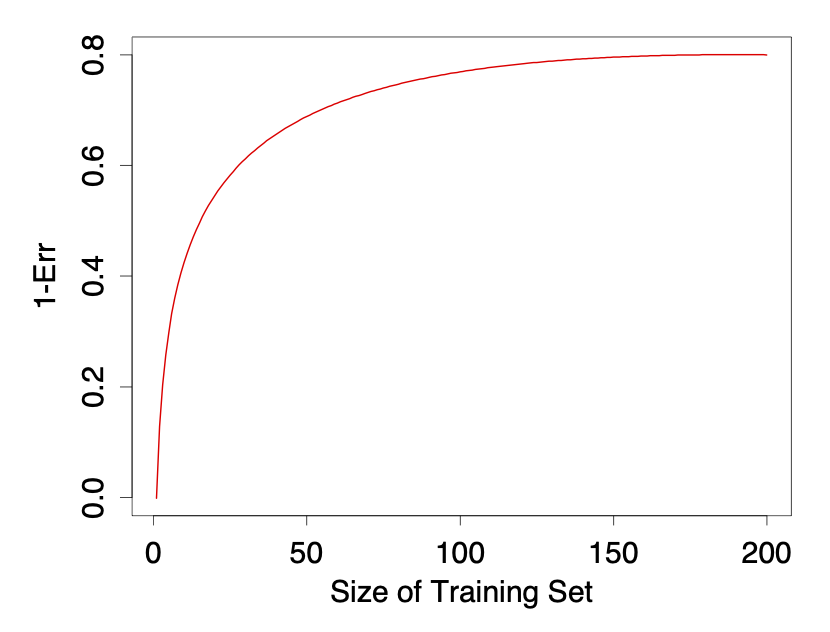
\includegraphics[width=0.7\textwidth]{figs/ESL_7_8.png}
\end{figure}

\end{frame}


\begin{frame}{K-fold Cross Validation}

\begin{itemize}
\item Common $K$ are: $K=\{2,5,10\}$
\item Smaller $K$ gives larger bias
\item Larger $K$ is computationally more costly
\item $K=10$ is a common approach
\end{itemize}

\end{frame}


\begin{frame}{Leave-One-Out Cross Validation}

\begin{itemize}
\item When $K=N$
\item Benefits
\begin{itemize}
\item Almost unbiased estimate of $\text{Err}$
\item Sometimes we only need to train our model once
\end{itemize}
\item Drawbacks
\begin{itemize}
\item Higher Variance in estimate of $\text{Err}$
\item Can be more computationally very costly (naive implementation)
\item Can be unstable/less robust in some settings
\end{itemize}
\end{itemize}

\end{frame}


\begin{frame}{Leave-One-Out Cross Validation}

\begin{figure}[h]
\caption{Cross-Validation Bias (Hastie et al, 2009, Fig. 7.14)}
\centering
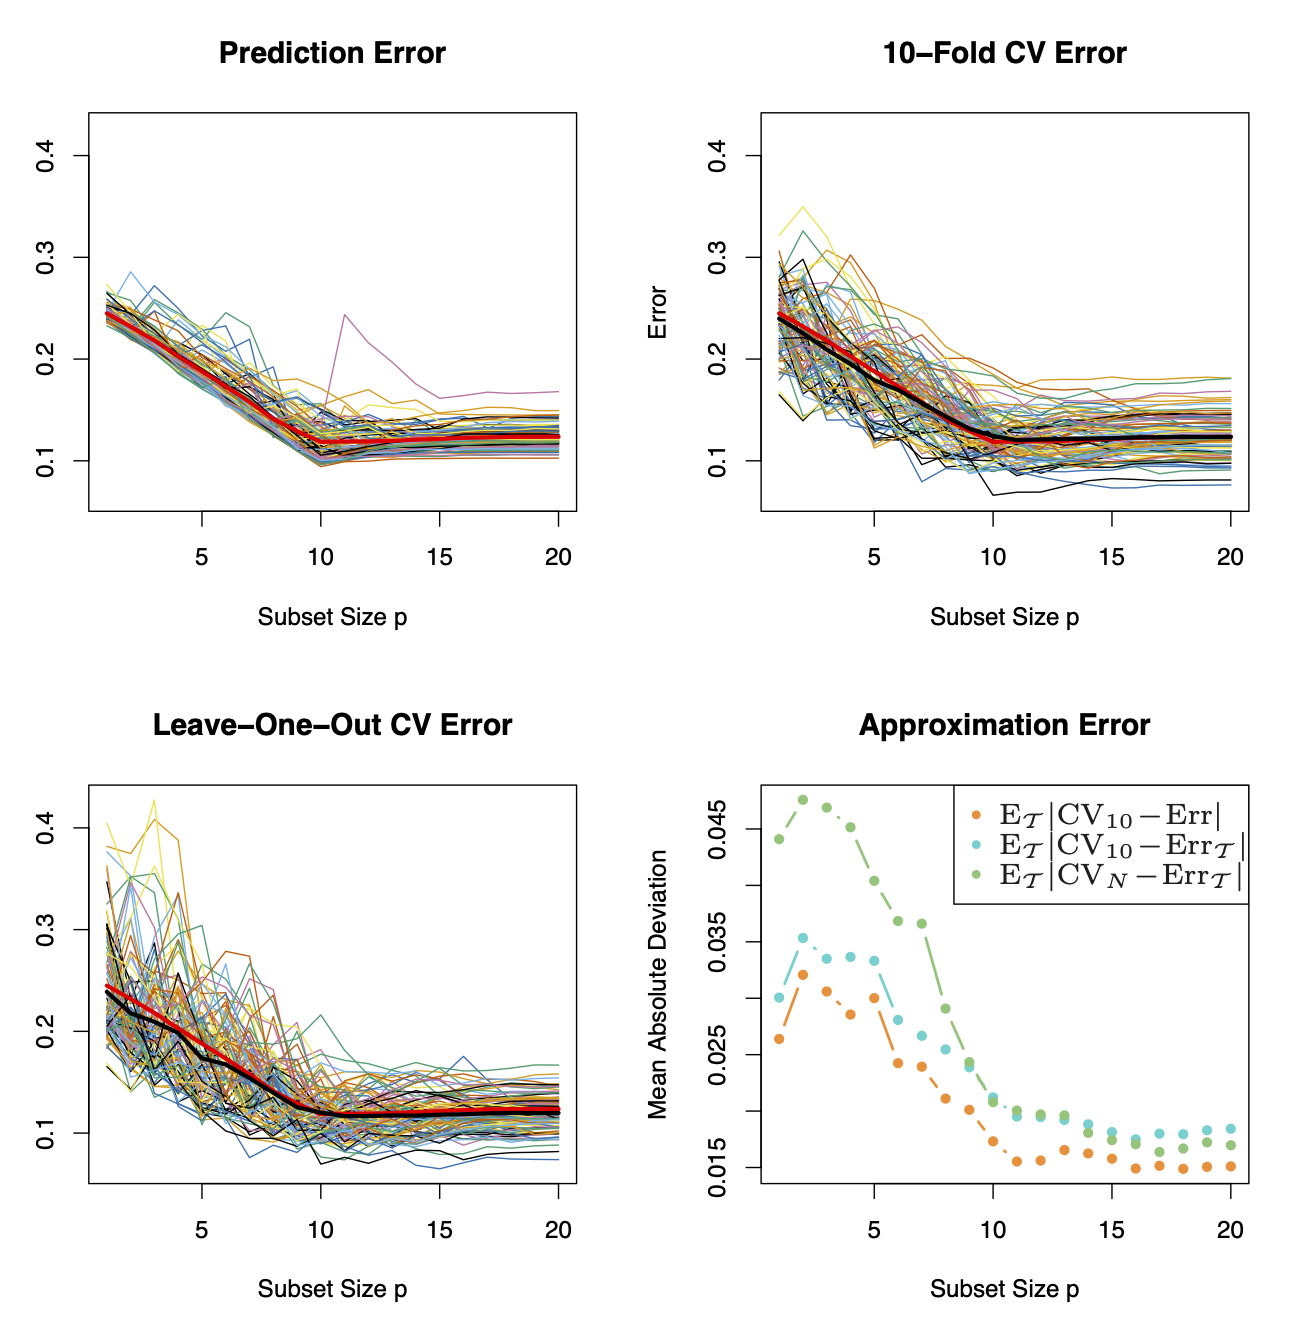
\includegraphics[width=0.7\textwidth]{figs/ESL_7_14.png}
\end{figure}

\end{frame}


% TODO: Add?

%\begin{frame}{LOO-CV for large data}

%\[
%CV(\hat{f},\alpha) = \frac{1}{N}\sum^N_{i=1} L(y_i,\hat{y}_{-\kappa(i)}(x_i,\alpha)
%\]

%Lets use sampling theory!\\[3mm]\pause

%Difference estimator

%Good approximations of the optimism.

%\end{frame}



\begin{frame}{The role of the data generating process}

\begin{itemize}
\item we assume that testset and train set are different observations from the same data generating process
\[
\mathbf{d} = \{(y_i, \mathbf{x}_i), i = 1, ..., n\} \,\sim P_{y,x}
\]
\item The (naive) assumption: independence
\item Things that can go wrong:
\begin{itemize}
\item temporal leak/concept drift
\item duplicated observations
\item non-randomized data
\end{itemize}
\pause
%\item Example: Evaluating prediction models for Elections
% TODO: Add examples from the bachelor theses
\end{itemize}


\end{frame}


\begin{frame}{Example: Election prediction}

\begin{itemize}
\item We want to predict the next election
\item We know that there are "\uured{concept drift}"
\item Solution in Frölander and Uddhammar (2021) and Olsson and Ölfvingsson (2021)
\begin{enumerate}
\item LOO-CV on the elections 1973-2014
\item The elections 2018 as the final validation set
\end{enumerate}


\end{itemize}

\begin{figure}[h]
\caption{Predictive distr. (Olsson and Ölfvingsson, 2021, Fig. 6)}
\centering
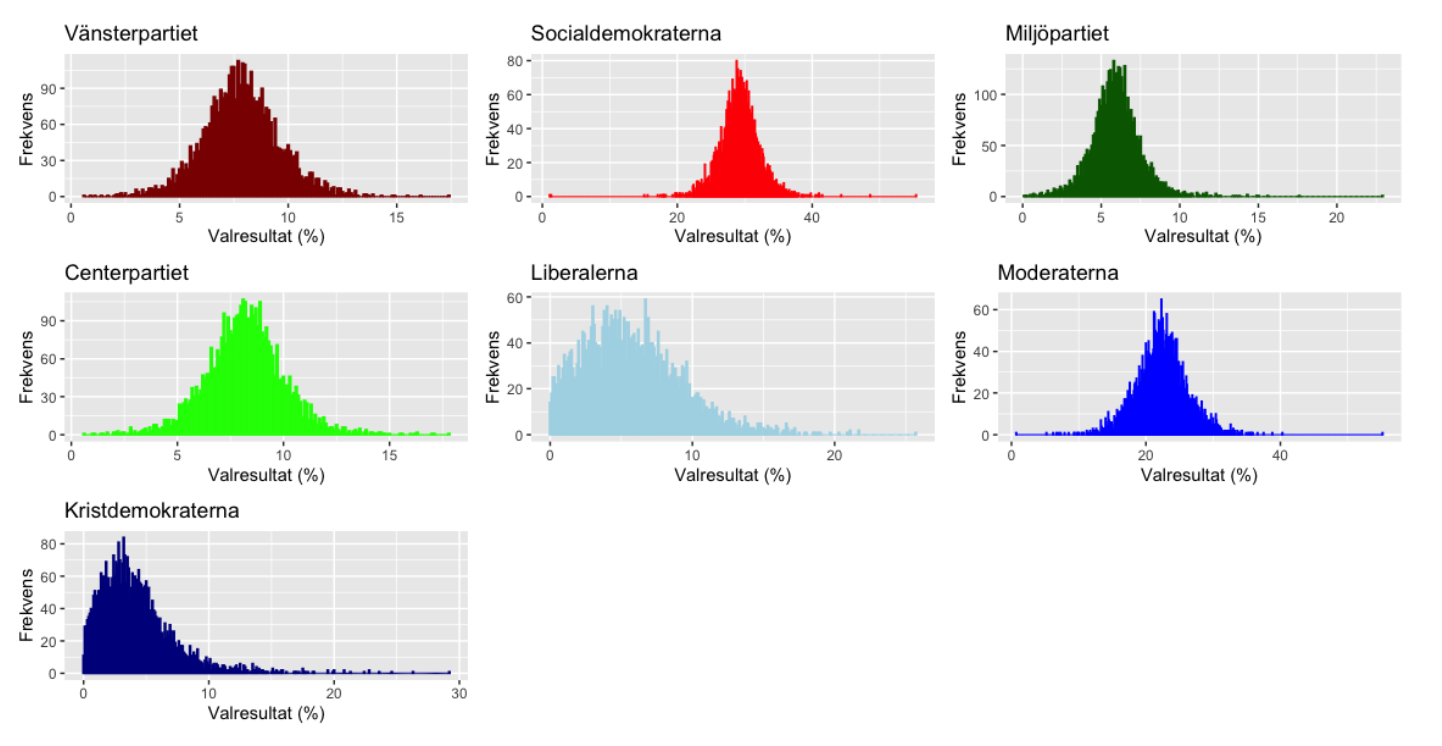
\includegraphics[width=1\textwidth]{figs/elections}
\end{figure}

\end{frame}


\begin{frame}{What is CV estimating?}

\begin{align*}
\text{Err} & = \E_{p(X,Y)} (\text{Err}_\mathcal{T})
\end{align*}

\begin{enumerate}
\item What do we want CV to estimate, $\text{Err}$ or $\text{Err}_\mathcal{T}$?
\pause
\item What is CV estimating?
\end{enumerate}

\end{frame}


\begin{frame}{What is CV estimating?}

Let $\text{Err}_{XY} = \text{Err}_\mathcal{T}$. Further, assume the true model is
\[
y_i = \mathbf{x}^T \theta + \epsilon_i
\]
where $\epsilon_i \sim N(0,\sigma^2)$.

\begin{figure}[h]
\caption{MSE and missclassification ($\alpha=10\%$, Bates et al, 2022)}
\vspace{-5mm}
\centering
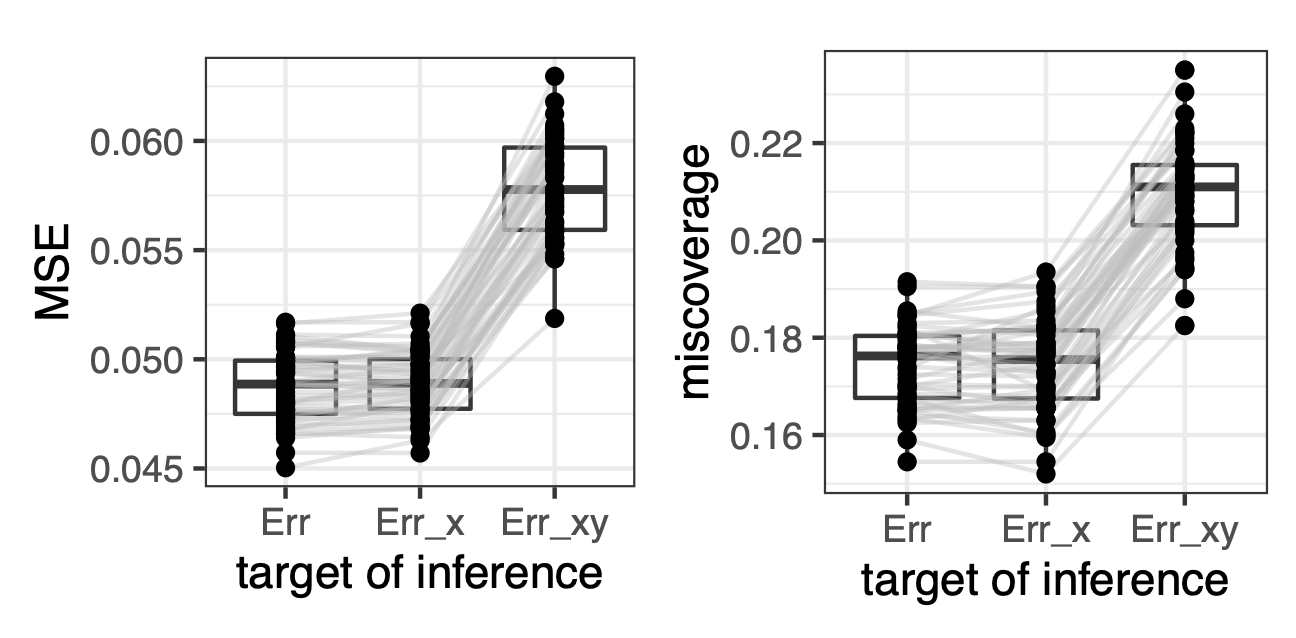
\includegraphics[width=0.75\textwidth]{figs/bales2021}
\vspace{-5mm}
\end{figure}
\pause
Two take-aways:
\vspace{-2mm}
\begin{enumerate}
\item CV is estimating $\text{Err}$ (see Bates et al, 2022)
\pause
\item Naive SE of CV estimators underestimate the true SE (see Bengio and Goodfellow, 2004)
\end{enumerate}


\end{frame}


\begin{frame}{Test error and (cross-)validation error?}

\begin{enumerate}
\item What is the difference between the validation and test error?
\pause
\item Why use cross-validation instead of holding out one validation fold?
\end{enumerate}

\end{frame}

\begin{frame}<handout:0>{Questions?}
Questions?
\end{frame}




%%%%%%%%%%%%%%%%%%%%%%%%%%%%%%%%%%%%%%%%%%%%%%%%%%%%%%%%%%%%%%%%%%

%\section{Regularisation}
%\frame{\sectionpage}

%\begin{frame}{Regression and GLM}
%\begin{itemize}
%\item Linear regression and logistic regression are examples of {\color{uured}generalised linear models}, GLMs.\\[3mm]\pause
%\item Both use maximum likelihood estimation for fitting the model, where the likelihood function $L(\beta)$ is maximised.
%\end{itemize}
%\end{frame}

%\begin{frame}{Regularised regression models}
%\begin{itemize}
%\item In some situations, for instance when the predictors are highly collinear, when there are too many predictors or when there is complete separation in the data, maximum likelihood estimation is unstable.\pause
%\begin{itemize}
%\item Either the solution is not unique, or minuscule changes in the data can change the solution completely.\pause
%\item Such datasets are increasingly common in e.g. genomics, finance, astronomy and image analysis.\\[3mm]\pause
%\end{itemize}

%\item In such cases, {\color{uured}regularisation/shrinkage methods} can be used instead.\\[3mm]\pause
%\item In a regularized GLM, it is not the likelihood $L(\beta)$ that is maximized, but a {\color{uured}regularised} function $L(\beta) \cdot p(\beta)$, where $p$ is a penalty function that typically forces the resulting estimates to be closer to 0, which leads to a stable solution.
%\end{itemize}
%\end{frame}

%\begin{frame}{Regularised regression models}
%Regularised linear regression models increase the {\color{uured}bias} of the estimates, but lowers their {\color{uured}variance}, thereby potentially decreasing the MSE.
%\end{frame}

%\begin{frame}{Connection to Bayesian estimation}
%In Bayesian estimation, a {\color{uured}prior distribution} $p(\beta)$ for the parameters $\beta_i$ is chosen.\\[3mm]\pause
%The estimates are then computed from the conditional distribution of the $\beta_i$ given the data, called the {\color{uured}posterior distribution}.\\[3mm]\pause
%Using Bayes' theorem, we find that
%$$P(\beta|\mathbf{x})\propto L(\beta)\cdot p(\beta),$$
%i.e. that the posterior distribution is proportional to the likelihood times the prior.\\[3mm]
%A special type of Bayesian estimator is the {\color{uured}maximum a posteriori (MAP)} estimator, which is found by maximizing the above expression (i.e. finding the mode of the posterior).\\[3mm]
%This is equivalent to the estimates from a regularised frequentist model with penalty function $p(\beta)$!
%\end{frame}

%\begin{frame}{Inference and invariance}
%\begin{itemize}
%\item Regularised regression models are not invariant under linear rescaling of the predictors.\pause
%\begin{itemize}
%\item If a predictor is multiplied by a scalar $a\neq 0$, this can change the entire model.\pause
%\item A model with measurements in inches might yield completely different results from a model with measurements in cm.\\[3mm]\pause
%\end{itemize}
%\item For this reason, it is widely agreed that the predictors should be standardized to have mean 0 and variance 1 before a regularised model is fitted.\pause
%\begin{itemize}
%\item With this approach we choose a particular (natural?) scaling, among all possible scalings.\pause
%\item All predictors are on the same scale and are therefore treated equally by the penalty function.\pause
%\end{itemize}
%\end{itemize}
%\end{frame}

%\begin{frame}{Inference and invariance}
%\begin{itemize}
%\item Hypothesis tests are available (e.g. Lockhart et al. (2014), A significance test for the lasso, \emph{Annals of Statistics}), but I advise against using them.\\[3mm]\pause
%\item Note that the hypothesis tests will be conditioned on the choice of scaling.\pause
%\begin{itemize}
%\item Because of this, regularised models are not appropriate for hypothesis testing -- the p-values could change completely if we rescaled the data!\\[3mm]\pause
%\end{itemize}
%\item Regularised regression models are however very useful for {\color{uured}predictive modelling}.
%\end{itemize}
%\end{frame}

%\begin{frame}{$L_q$-penalties}
%The most popular penalty terms correspond to common {\color{uured}$L_q$-norms}. \pause On a log-scale, the function to be maximized is
%$$\ell(\beta)+\lambda\sum_{i=1}^p|\beta_i|^q,$$
%where $\ell(\beta)$ is the loglikelihood of $\beta$ and $\sum_{i=1}^p|\beta_i|^q$ is the $L_q$-norm, with $q\geq 0$.\\[3mm]\pause
%This is equivalent to maximizing $\ell(\beta)$ under the constraint that $\sum_{i=1}^p|\beta_i|^q\leq\frac{1}{h(\lambda)}$, for some increasing positive function $h$.\pause
%\begin{itemize}
%\item Relies on the {\color{uured}sparsity} assumption that most $\beta$ are 0.\\[3mm]\pause
%\end{itemize}
%$\lambda\geq 0$ is a {\color{uured}smoothing parameter}:
%\begin{itemize}
%\item When $\lambda=0$, we are back at the standard ML-estimate.
%\item The $\hat{\beta}$ are forced to be closer to 0 when $\lambda$ increases.
%\item $\lambda$ is usually chosen using cross-validation.
%\end{itemize}
%\end{frame}


%\begin{frame}{Ridge regression}
%When the $L_2$ penalty is used, the regularised model is called {\color{uured}ridge regression}, for which we maximize
%$$\ell(\beta)+\lambda\sum_{i=1}^p\beta_i^2.$$
%\begin{itemize}
%\item Invented and reinvented by several authors, from the 1940's onwards.\\[3mm]\pause
%\item In a linear model, the OLS estimate is $\hat{\beta}=(\mathbf{X}^T\mathbf{X})^{-1}\mathbf{X}^T\mathbf{y}$, whereas the ridge estimate is $\hat{\beta}=(\mathbf{X}^T\mathbf{X}+\lambda \mathbf{I})^{-1}\mathbf{X}^T\mathbf{y}$. The $\lambda \mathbf{I}$ is the 'ridge'.\\[3mm]\pause
%\item The $\beta_i$ can become very small, but are never pushed all the way down to 0.\\[3mm]\pause
%\item In a Bayesian context, this corresponds to putting a standard normal prior on the $\beta_i$.
%\end{itemize}
%\end{frame}

%\begin{frame}{Lasso}
%When the $L_1$ penalty is used, the regularised model is called the {\color{uured}lasso} (Least Absolute Shrinkage and Selection Operator), for which we maximize
%$$\ell(\beta)+\lambda\sum_{i=1}^p|\beta_i|.$$
%\begin{itemize}
%\item Introduced by Robert Tibshirani in 1996.\\[3mm]\pause
%\item As $\lambda$ increases, more and more $\beta_i$ become 0.\pause
%\begin{itemize}
%\item Simultaneously performs estimation and variable selection!\\[3mm]\pause
%\end{itemize}
%\item In a Bayesian context, this corresponds to putting a standard Laplace prior on the $\beta_i$.
%\end{itemize}
%\end{frame}

%\begin{frame}{Examples in R}
%Functions for regularised generalized linear models (linear, logistic, Poisson, multinomial, and more) are available e.g. in the \texttt{glmnet} package for R.\\[3mm]\pause
%The syntax used is somewhat different from that for \texttt{glm} and \texttt{lm}.\\[3mm]
%\end{frame}


%\begin{frame}{Generalizations}
%Regularised models have been a hot research topics in the last 20 years. Some additional important models are:\pause
%\begin{itemize}
%\item {\color{uured}Elastic net:} a compromise between ridge and lasso, in which $$\ell(\beta)+\lambda_1\sum_{i=1}^p|\beta_i|+\lambda_2\sum_{i=1}^p\beta_i^2$$ is maximized.\pause
%\begin{itemize}
%\item Introduced by Zou and Hastie in 2005.\pause
%\item Is better than the lasso at handling correlated predictors.\pause
%\item Has two smoothing parameters that we need to choose.\pause
%\item Available in the \texttt{glmnet} package.\\[3mm]\pause
%\end{itemize}
%\item {\color{uured}Group lasso:} a version of the lasso in which variables can be grouped before fitting the model. The group lasso then selects groups of variables rather than individual variables.\pause
%\begin{itemize}
%\item Introduced by Yuan and Lin in 2006.\pause
%\item Useful e.g. when we have dummies for categorical variables (in contrast, the lasso may choose to only include the dummies for some of the categories).
%\end{itemize}
%\end{itemize}
%\end{frame}






\end{document}
